\newpage
\section{Proposed Power System Design (Problem 5, 6)\footnote{Problem 5 and 6 were combined as explaining the thruster configuration and the single line diagram independently lead to repeating a lot of the same arguments}} \label{prob_5and6}

% \todo[inline]{Things that \textbf{have to} be answered \\     \begin{itemize}
%     \item Include the diagram for the propulsion system/segregations 
%     \item Disuse the segregations for the power \textbf{and} the thruster system
%         \subitem{Thrusters}
%         \subitem{Feeders cables}
%         \subitem{Gensets}
%         \subitem{Machine rooms}
%         \subitem{Sectioning of main switchboard}
%         \subitem{Requirements for the bus-tie breakers}
%     \item Include our SLD
%     \item Explain the worst-case failure based on our SLD
%     \item Explain how our design still provides the required propulsion power
% \end{itemize}}

\subsection{Introduction}
\subsubsection{The design philosophy}\label{Sec:designPhilosophy}
The philosophy when designing the power system and the thruster configuration was most off all to make a system that is realistic, in accordance to the applicable standards and what is used in the industry. If a DP system fail it can lead to hazards and serious consequences. Therefore, effort was putt into making the system more reliable than the minimum requirements and this includes multiple levels of redundancy. In order to make the system as realistic as possible, it was also decided to try to make sure the equipment that was used in the project was available in the market today. Also, the load level on the generators were considered in order to make them work within a reasonable load level. However, it was not necessary to do that with the thrusters, since its power demand was given, thus out of the scope of the project. 


\subsubsection{Industry Practices} \label{Sec:industryPractices}
Based on the single-line diagrams and thruster configurations of semi-submersibles used today, it can be seen that the most common arrangement is to use four redundancy groups for the generation and one to two thrusters placed in each corner of the pontoons. These kind of configurations can be seen in the example configuration from the lecture notes and the diagram for the semi-sub "DEEPWATER HORIZON" found in Appendix \ref{Sec:ThrusterConfiguratons}.  

\subsubsection{Design requirements} \label{Sec:designRequirements}
As summary of the requirements given in the problem description is summed up in Table \ref{tab:designRequirements}. It was assumed that the service load during worst-case failure stayed the same at 4MW, the same as during single failure. The service loads under normal operation was assumed to be three times that of the single failure load, so totally 12MW.  

\begin{table}[h]
    \centering
    \begin{tabular}{l c c}
                        & \text{Normal Operation [MW]} & \text{Worst-case Failure [MW]}  \\
    \toprule
    \text{Propulsion Power}     & 42                   &  34  \\
    \text{Service Loads}        & 12                   &  4  \\
    \text{Drilling Power}       & 12                   &  0  \\
    \midrule
    \text{Total Loads}          & 66                   &  38 \\
    \bottomrule
    \end{tabular}
    \caption{Design requirements}
    \label{tab:designRequirements}
\end{table}



\subsubsection{Definition of worst-case failure} \label{Sec:worstCaseFailure}
DNV GL definition of worst case failure is explained in Section \ref{Sec:3d}. In short, it states that DNV GL defines the worst-case failure as the (single) failure that causes the loss of the most significant redundancy group. In this case, that would correspond to loosing one redundancy group. However, there might be worse scenarios, and since a failure of a DP system on a rig would have potentially significant consequences. Therefore, to lower the risk levels (environmental, to human life or financial), it is desirable that the system is more redundant than the minimum requirement. In order to ensure that, the rig was designed such that it would also be able to hold its position if two redundancy groups were out of service. This was defined as this rig's worst case failure condition and is that is mean when the term \textit{worst-case failure} is used for the rest of the report. 

\subsection{The System Design}
\subsubsection{Layout}
Under normal DP operation, it is common practice to have at least one thruster in each corner in operation \cite{RedundantDesignIntention_DNV}.
This improves the rig's maneuverability, therefore its capability of holding itself in place. A standard redundancy measure would therefore be to have at least two thrusters in each corner. This is consistent with what is normal industry practice as described before. This configuration can for example be seen used for the "DEEPWATER HORIZON" which can be found in Appendix \ref{Sec:ThrusterConfiguratons}. 

 \begin{figure}[h!]
 	\centering
	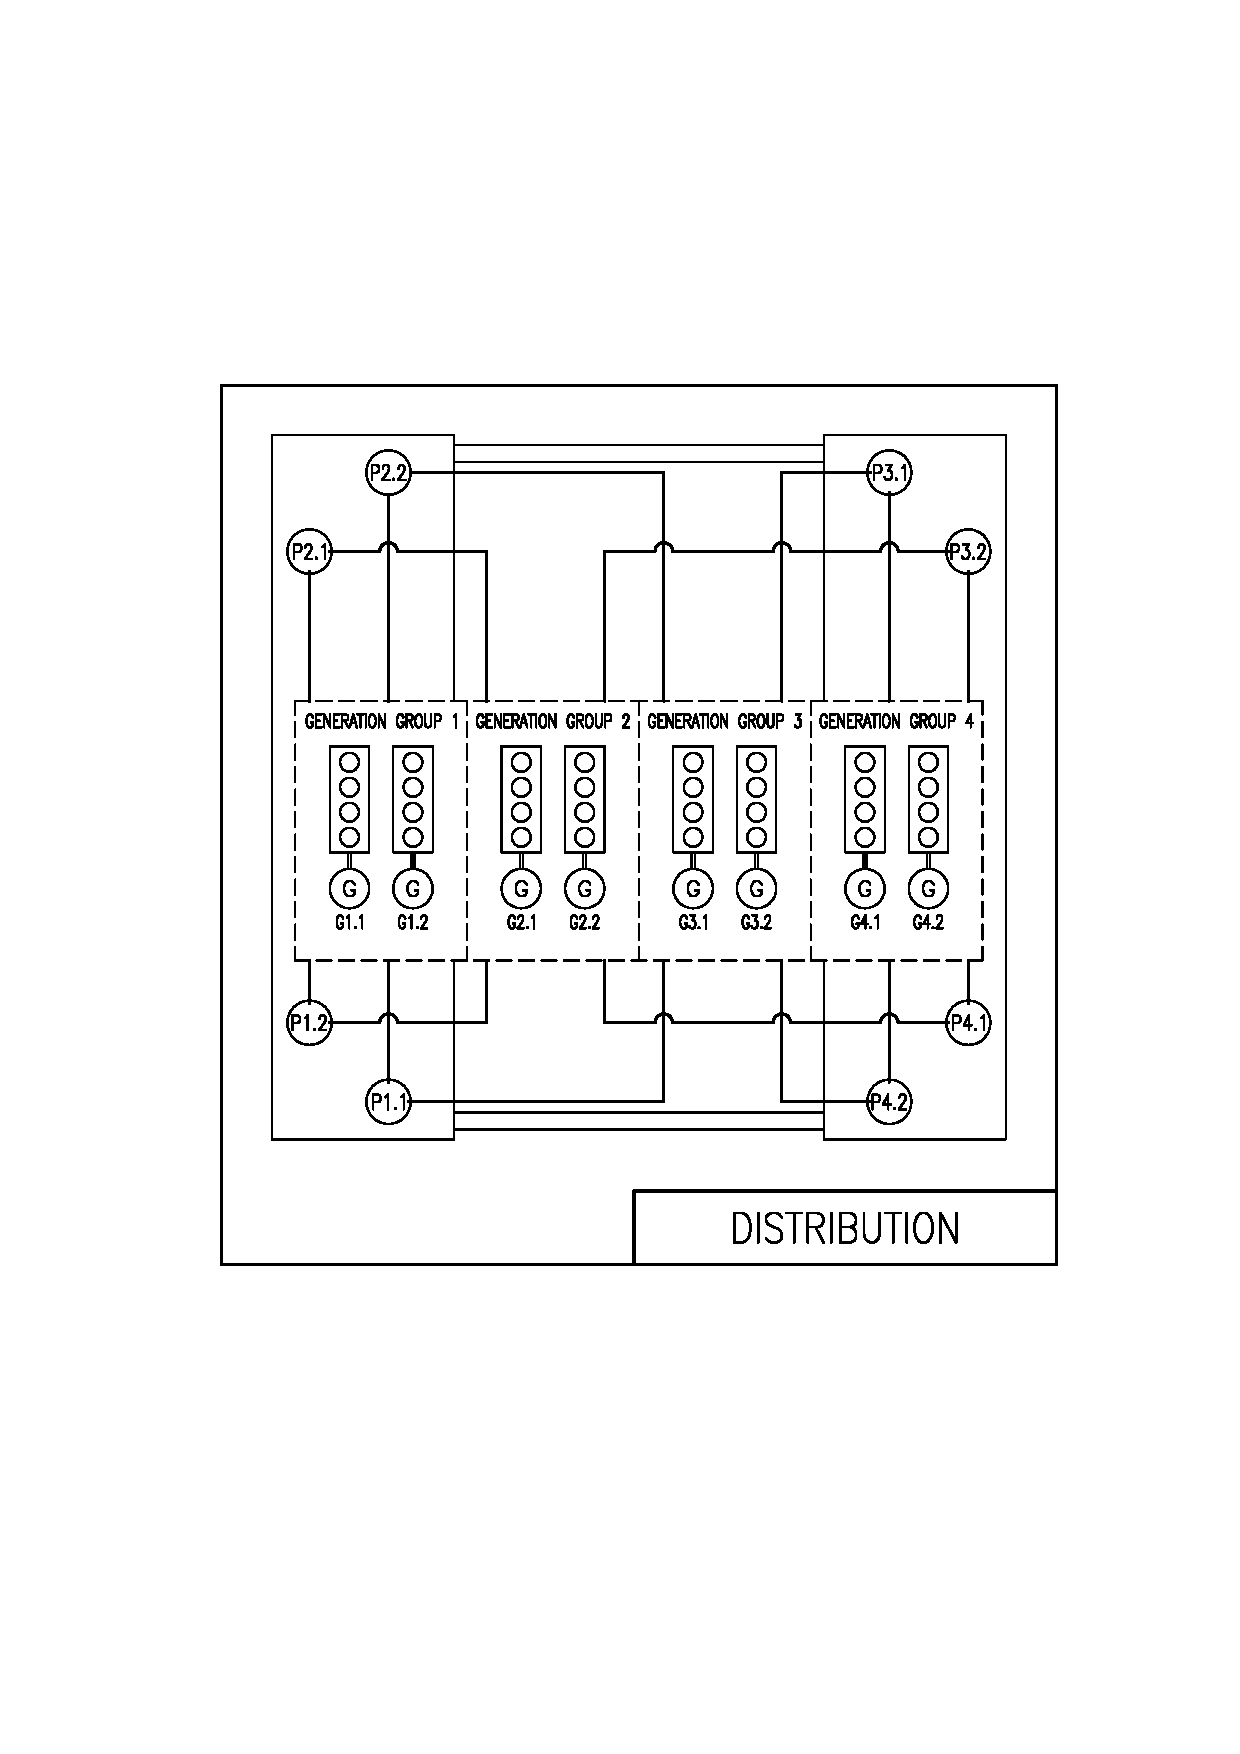
\includegraphics[width = 10cm]{figures/Single_Line_distribution.pdf}
	\caption{Thruster and generator group distribution}
	\label{fig:ThrusterAndGeneratorGroupDistribution}
\end{figure}	

The thruster configuration for the designed proposed in this report can be found in Figure \ref{fig:ThrusterAndGeneratorGroupDistribution}. As can be seen in the figure, the design follows the industry practice of two propulsion units in each corner, where the propulsion units are all connected to two separate generator groups. Using this design, no failure of any two compartments can cause the loss of both thrusters in one corner of the rig. This ensures that the rig has good maneuverability also during the defined worst-case failure condition and thereby provides the desired reliability. The connections between the propulsion units and the generator groups is summarized in Table \ref{tab:genGroupToThruster}, making the results of each possible failure condition easier to visualize.   

\begin{table}[H]
    \centering
    \begin{tabular}{l|cc|cc|cc|cc}
    \text{Propulsion units:} & P1.1 & P1.2 & P2.1 & P2.2 & P3.1 & P3.2 & P4.1 & P4.2 \\
    \hline
    %\toprule
    \text{Generation group 1} & X & X & X & X &   &   &   &    \\
    \text{Generation group 2} &   & X & X &   &   & X & X &    \\
    \text{Generation group 3} & X &   &   & X & X &   &   & X\\
    \text{Generation group 4} &   &   &   &   & X & X & X & X  \\
    \end{tabular}
    \caption{Generation-group-to-propulsion-units connections}
    \label{tab:genGroupToThruster}
\end{table}

\begin{figure}[h]
    \centering
    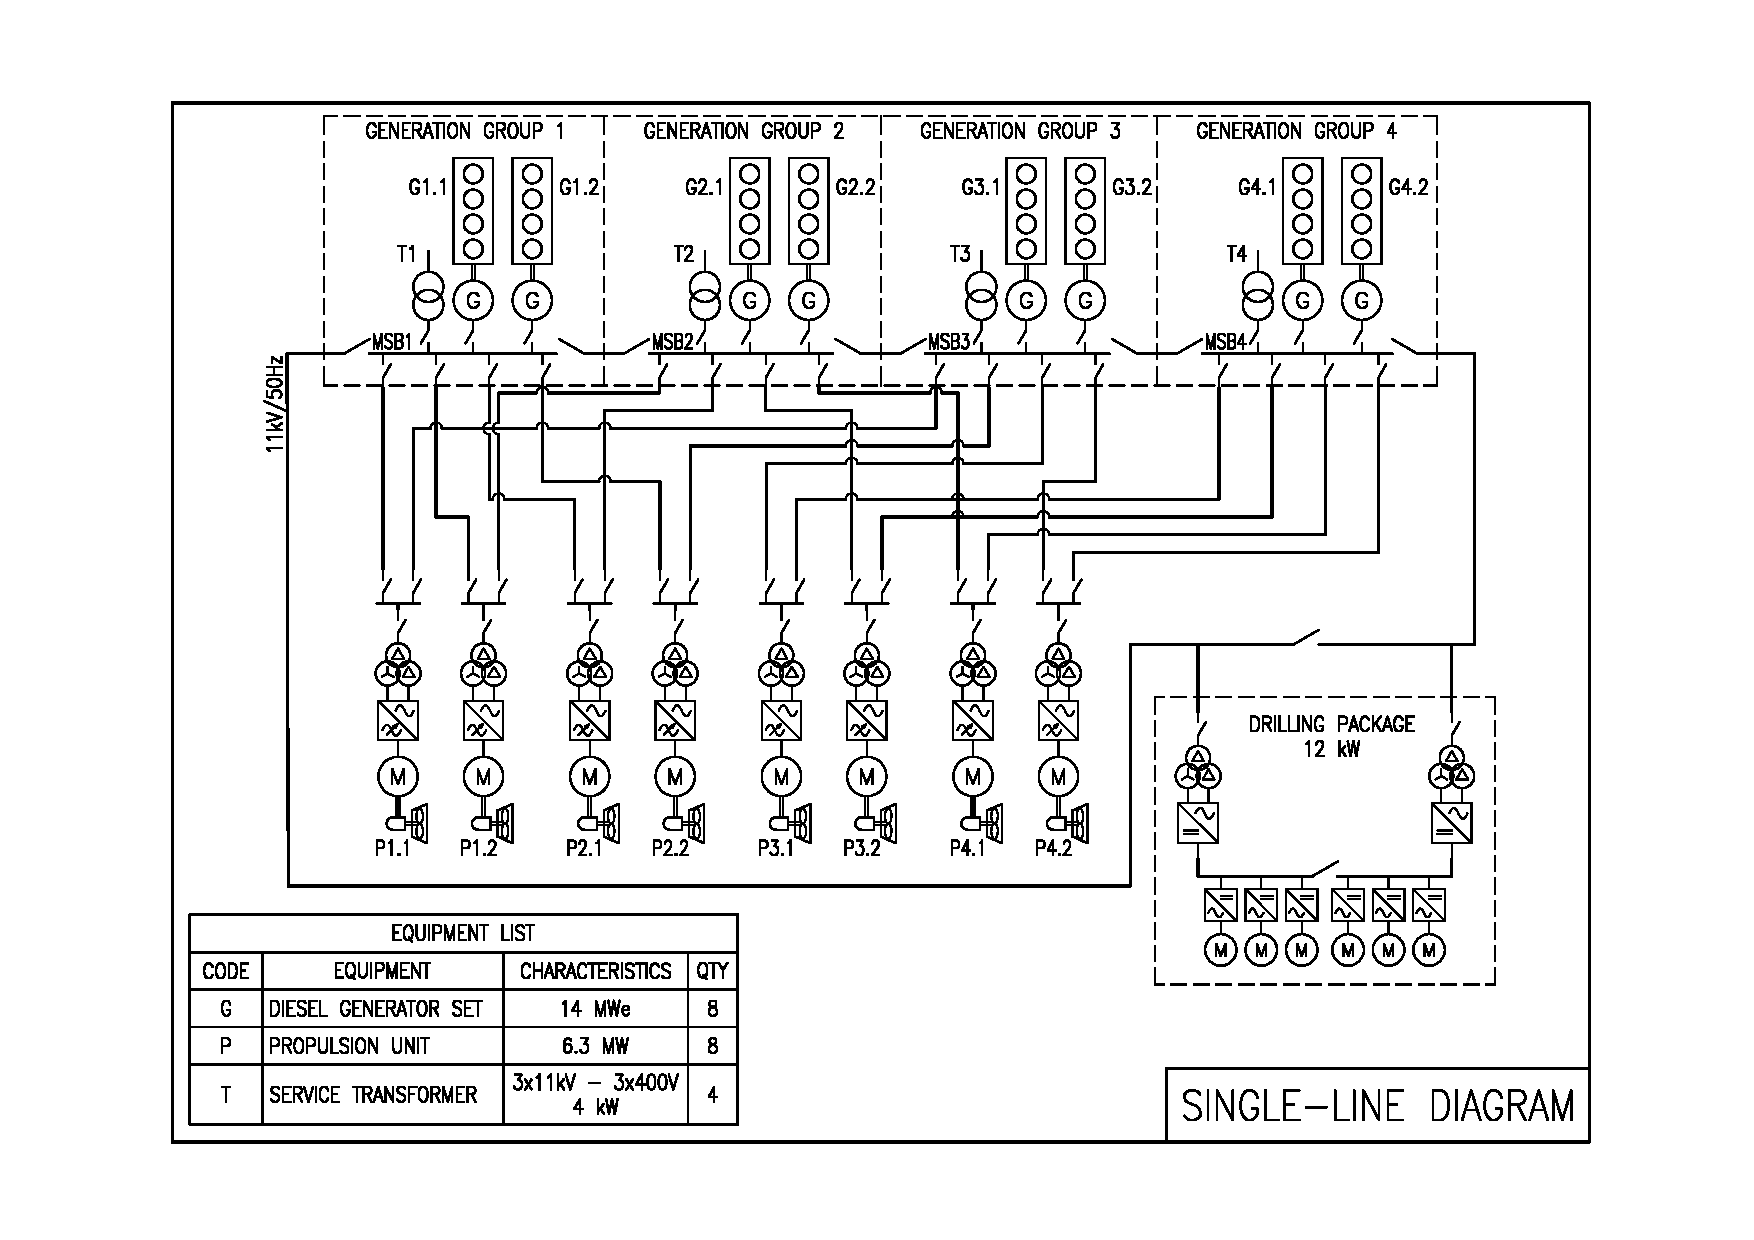
\includegraphics[width = \textwidth]{figures/Single_Line_diagram.pdf}
    \caption{Single line diagram of the system}
    \label{fig:SingleLineDiagram}
\end{figure}

\todo{See that there is a reference problem the single line diagram is referred as figure 6 just next to the same figure 2. may be we should refer to 2 figures?}

The separation into the different redundancy groups is visualized in the single line diagram in Figure \ref{fig:SingleLineDiagram}. The system is comprised of four separated redundant generator groups, each consisting of two 14MW generators, one 4MW distribution transformer and one main switchboard. Each of the switchboards can be connected in a ring configuration by closing the breakers seen in the diagram.     

\subsection{Dimensions of the components}
In order to dimension the system in such a way that it satisfies the design criteria, certain calculations had to be done and which were repeated in an iterative manner. Note, the choice of voltage on the main switchboard is explained in Section \ref{sec:8a)} and the size chosen for the distribution transformers is further explained in Section \ref{sec:8b)}. The size of the thrusters are further explained in Section \ref{sec:8e)} 

\subsubsection{The Generators}
After looking at the industry practices and considering the desired level of redundancy, it was decided to have two gensets present in each generation group. That way, failure in one of them would not lead to failure of a whole group, adding a second level of redundancy. 

With this in mind, the next step was to determine the rating of the gensets in order to supply the required power to the drilling and propulsion system, as well as the distribution transformer, also accounting for the losses on the components of the system. These calculations were done both for the normal operation condition and the worst-case failure condition. The efficiencies used are summed up in Table \ref{tab:efficiencies} and the calculation of the total required generated power for both conditions can be found in Table \ref{tab:powerDemand}.

\begin{table}[h!]
    \centering
    \begin{tabular}{l l}
        \text{Component} & \text{Efficiency} \\
        \toprule
        \text{Switchboard ($\eta_s$)}         & $\eta_s$ = 0.999  \\
        \text{3-Phase Transformer ($\eta_t$)} & $\eta_t$ = 0.993  \\
        \text{Frequency Converter ($\eta_f$)} & $\eta_f$ = 0.985  \\
        \text{Electric Motor ($\eta_m$)}      & $\eta_m$ = 0.960  \\
    \bottomrule
    \end{tabular}
    \caption{Efficiency individual components \cite{LectureNote11PowerSystemDesign}}
    \label{tab:efficiencies}
\end{table}

\begin{table}[H]
    \centering
    \begin{tabular}{l r r r}
    & \text{Efficiency calculation [-]} & \text{Normal Operation [MW]} & \text{Worst-case Failure [MW]}  \\
    \toprule
    \rule{0pt}{12pt}\text{Propulsion}     & $\eta_p  = \eta_s^2\cdot\eta_t\cdot\eta_f\cdot\eta_m  = 0.937$ & $\frac{1}{\eta_p}\cdot$42  = 44.84  & $\frac{1}{\eta_p}\cdot$34 = 36.30   \\
    \rule{0pt}{12pt}\text{Service load}        & $\eta_{sl} = \eta_s  = 0.999$     & $\frac{1}{\eta_{sl}}\cdot$12 = 13.01  & $\frac{1}{\eta_{sl}}\cdot4$ =  4.00 \\
    \rule{0pt}{12pt}\text{Drilling}       & $\eta_d  = \eta_s^2 \cdot\eta_t\cdot\eta_f^2\cdot\eta_m = 0.923$   & $\frac{1}{\eta_d}\cdot$12 = 13.00  & 0   \\
    \midrule
    \text{Total}          &     & 69.86  & 40.30  \\
    \bottomrule
    \end{tabular}
    \caption{Power demand from the generators}
    \label{tab:powerDemand}
\end{table}

Knowing the required power, the rating of the gensets was adopted by calculating the load level on them, which should be on the range between 70 and 90\%, in order not to overload the gensets or to made them run in a low efficiency point either in any of the different scenarios:normal operation and worst-case failure power demands. This is shown in Table \ref{tab:powerDemand}. A generator size of 14MW was adopted and the loads for the scenarios are found in Table \ref{tab:gensetLoad}. This size generators ensured a very reliable system, as the load on the generators are good both if 6 or 7 gensets are running during normal operation, meaning that one genset can be in stand-by. Similarly, in the worst-case failure condition the four available gensets operates at only 71.97\% load and from the table it can be seen that it is also possible to operate with only three gensets in worst-case failure condition. 

\begin{table}[H]
    \centering
    \begin{tabular}{l l l l l l l}
        \text{Number of gensets in service} & 3 & 4 & 5 & 6 & 7 & 8 \\
        \toprule
        \text{Normal Operation (66MW)}   & - & - & - & 83.16\% & 71.29\% & 62.37\% \\
        \text{Worst-case failure (38MW)}  & 95.96\% & 71.97\% & 57.58\%\footnote{Only 1 failed compartment} &  47.98\%\footnote{Only 1 failed compartment} & - & - \\
        \bottomrule
    \end{tabular}
    \caption{Load on 14MW gensets}
    \label{tab:gensetLoad}
\end{table}

Finally, for the normal operation condition, the generators will have to supply a minimum of 69.86MWe. The total available power, 8 gensets of 14MWe rating, will be 112MWe. Such a high surplus is due to the redundancy level needed. 

For the worst-case failure condition, the generators will have to supply 40.30MWe power. In this case two generation groups are considered out of service, then the available power will be 56MW, which means that the generators will be able to supply the power at a load of 72\%.
